%!TEX root = ../TAMUTemplate.tex
%%%%%%%%%%%%%%%%%%%%%%%%%%%%%%%%%%%%%%%%%%%%%%%%%%%
%
%  New template code for TAMU Theses and Dissertations starting Fall 2016.
%
%  Author: Sean Zachary Roberson
%    Version 3.16.09
%  Last updated 9/12/2016
%
%%%%%%%%%%%%%%%%%%%%%%%%%%%%%%%%%%%%%%%%%%%%%%%%%%%

%%%%%%%%%%%%%%%%%%%%%%%%%%%%%%%%%%%%%%%%%%%%%%%%%%%%%%%%%%%%%%%%%%%%%%%
%%%                           SECTION II
%%%%%%%%%%%%%%%%%%%%%%%%%%%%%%%%%%%%%%%%%%%%%%%%%%%%%%%%%%%%%%%%%%%%%%

\chapter{\uppercase {Theoretical Framework}}
\label{ch:theoretical_framework}

This chapter will discuss the theoretical underpinnings of 


\section{The Standard Model}

Electromagnetism 1930 Herman Weyl~\cite{Weyl1929}.
	described as local symmetry represented by the Lie group U(1)

1954, Yang and Mills~\cite{PhysRev.96.191}.
	Gauge theory SU(2)
	electroweak

1970s strong force added using SU(3) group to describe color interactions

Combined to form
\begin{equation}\label{eq:standard_model_groups}
SU\left(3\right)_{C}{\otimes}SU\left(2\right)_{L}{\otimes}U\left(1\right)_{Y}
\end{equation}
$SU\left(3\right)_{C}$ describes colored QCD interactions
$SU\left(2\right)_{L}$ for weak interactions among quarks and leptons
$U\left(1\right)_{Y}$ for electromagnetic interactions

SM is a quantum field theory (QFT)


Since the mid-1970s, the Standard Model (SM) of particle physics has been the leading theory describing three of the four known fundamental forces (not including gravity) as well as classifying all of the known elementary particles.
In 1961 Sheldon Glashow combined the electromagnetic and weak interactions in the first step towards creating the SM~\cite{GLASHOW1961579}.
Steven Weinberg and Abdus Salam~\cite{PhysRevLett.19.1264,salam} continued this work by adding in the Higgs mechanism~\cite{PhysRevLett.13.321,PhysRevLett.13.508,PhysRevLett.13.585} (more on this later) in 1967.
The model entered its current form in 1973-1974 with the introduction of the strong force and quantum chromodynamics.
The model can be broken down into the matter particles, spin $\frac{1}{2}$ fermions called leptons and quarks, the force mediators, spin 1 gauge bosons, and the spin-0 mediator of the Higgs field, all of which can be found in figure~\ref{fig:standard_model}.
Even during it's formative years, the SM's success at predicting new particles (i.e. the top quark in 1995) and describing the properties of known particles (i.e. $W^{\pm}$ to $Z^{0}$ mass ratio) is undeniable.


\begin{figure}[!hbt]
	%\scalebox{.45}{\input{StandardModel}}
	\centering
	\resizebox{0.95\textwidth}{!}{\input{StandardModel_CERNWebfest2012}}
	\caption{The Standard Model of particle physics. The model includes three generations of matter particles (leptons and quarks) as well as the gauge and Higgs bosons.}
	\label{fig:standard_model}
\end{figure}

\section{Quantum Electrodynamics}
\section{Electroweak Interaction}
\section{Strong Interaction}
\section{Higgs Mechanism}


\begin{figure}[!hbt]
    \centering
    \begin{subfigure}[t]{0.48\textwidth}
        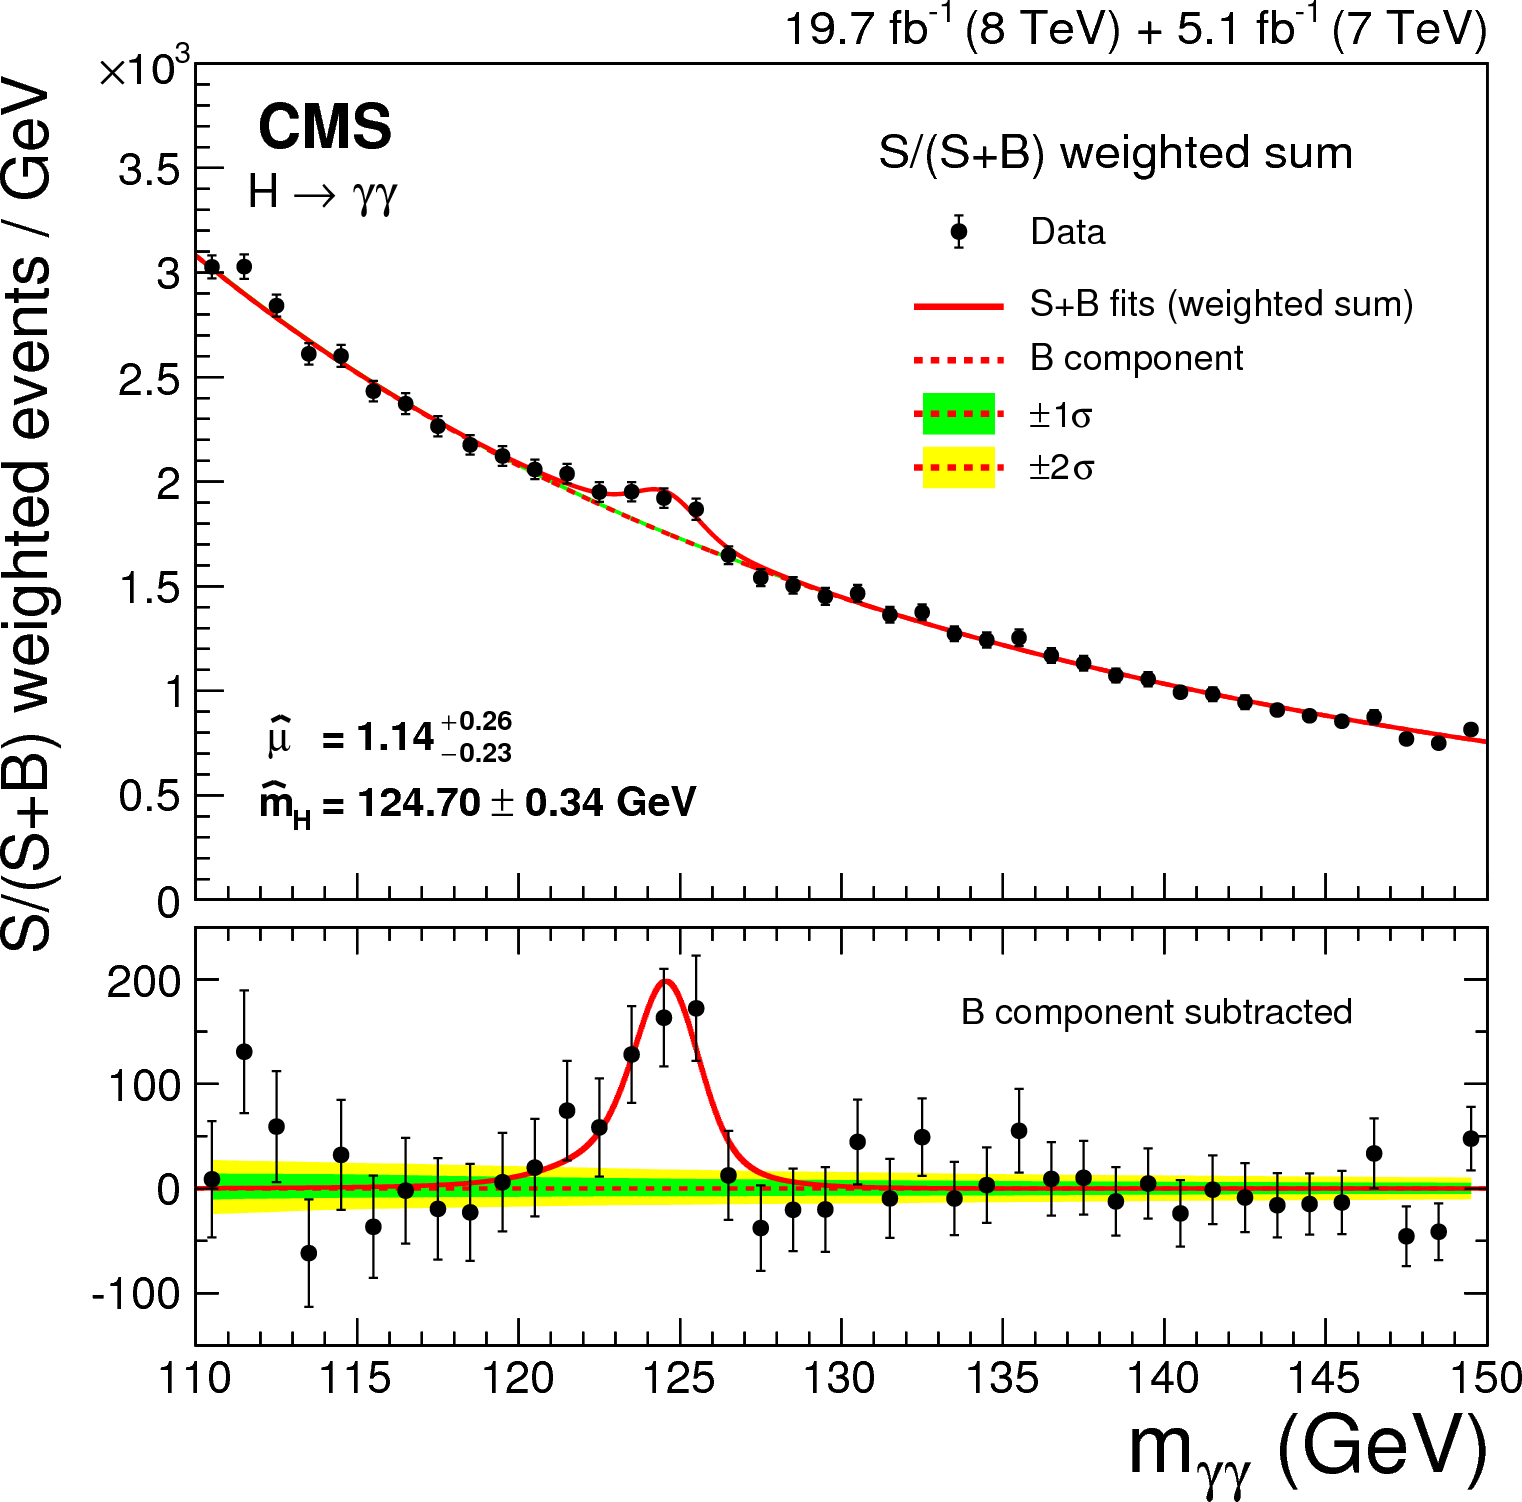
\includegraphics[width=\textwidth]{\figpath/Chapter2/HgammagammaPeak.png}
        \caption{}
        \label{fig:HgammagammaPeak}
    \end{subfigure}
    \begin{subfigure}[t]{0.48\textwidth}
        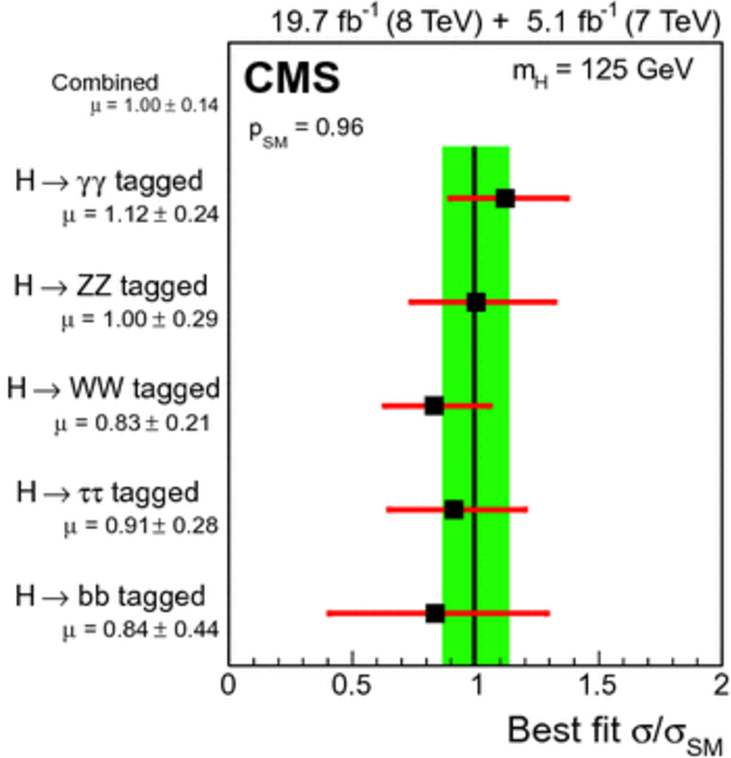
\includegraphics[width=\textwidth]{\figpath/Chapter2/10052_2015_3351_Fig4_HTML.pdf}
        \caption{}
        \label{fig:HiggsSignalStrength}
    \end{subfigure}
    \caption{(Left) The $H\rightarrow\gamma\gamma$ signal peak as seen in 2012~\cite{Hgammagamma}. (Right) Best-fit $\sigma/\sigma_{SM}$ grouped by predominant decay mode. The vertical band is the overall combined analysis value and the horizontal bars show the $\pm$1 uncertainties (statistical and systematic)~\cite{Khachatryan2015}.}
    \label{fig:HiggsIn2012}
\end{figure}

%, as seen in figure~\ref{fig:Higgs_WW_lnujj_feynman}

%While at 125\gev the gluon-gluon fusion (ggF) production cross section\footnote{This analysis is independent of production mode, but selects for a specific decay channel.} and $l\nu{qq}$ branching ratio are high, as seen in figure~\ref{fig:Higgs_XS_and_BR}, there are significant experimental challenges to overcome.


\begin{figure}[bt]
	\centering
	\begin{subfigure}[t]{0.415\textwidth}
		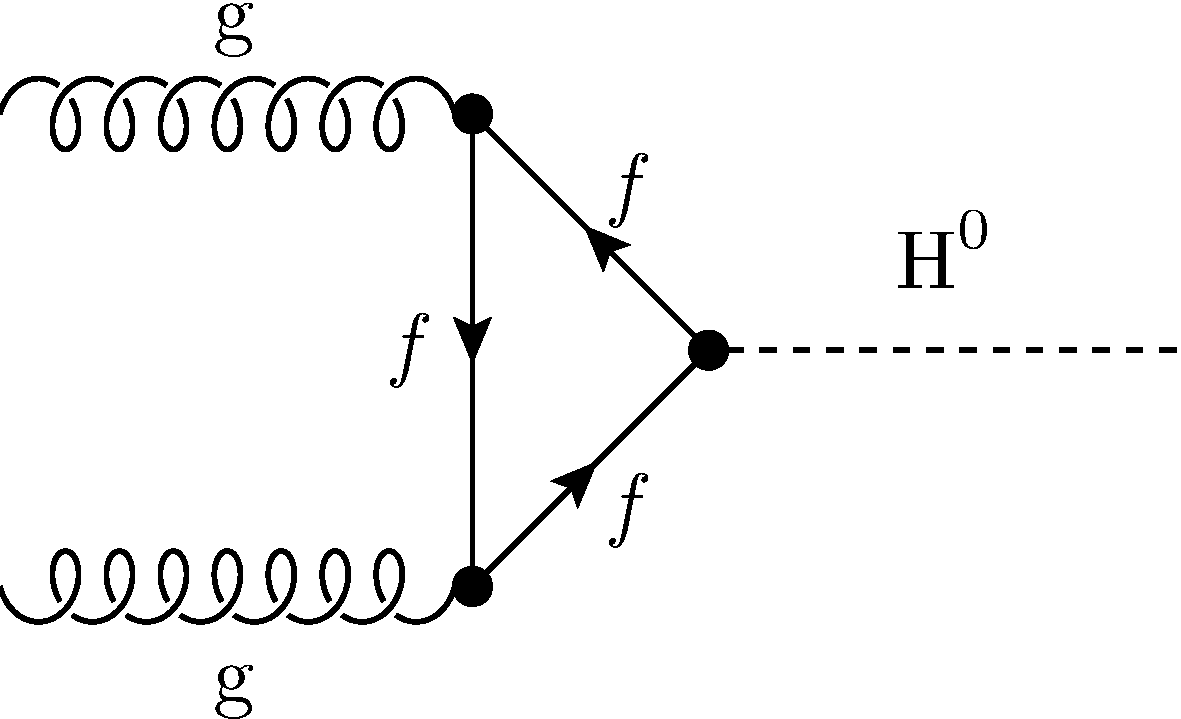
\includegraphics[width=\textwidth]{\figpath/FeynmanDiagrams/ggH.eps}
		\label{fig:ggH}
	\end{subfigure}%
	\begin{subfigure}[t]{0.415\textwidth}
		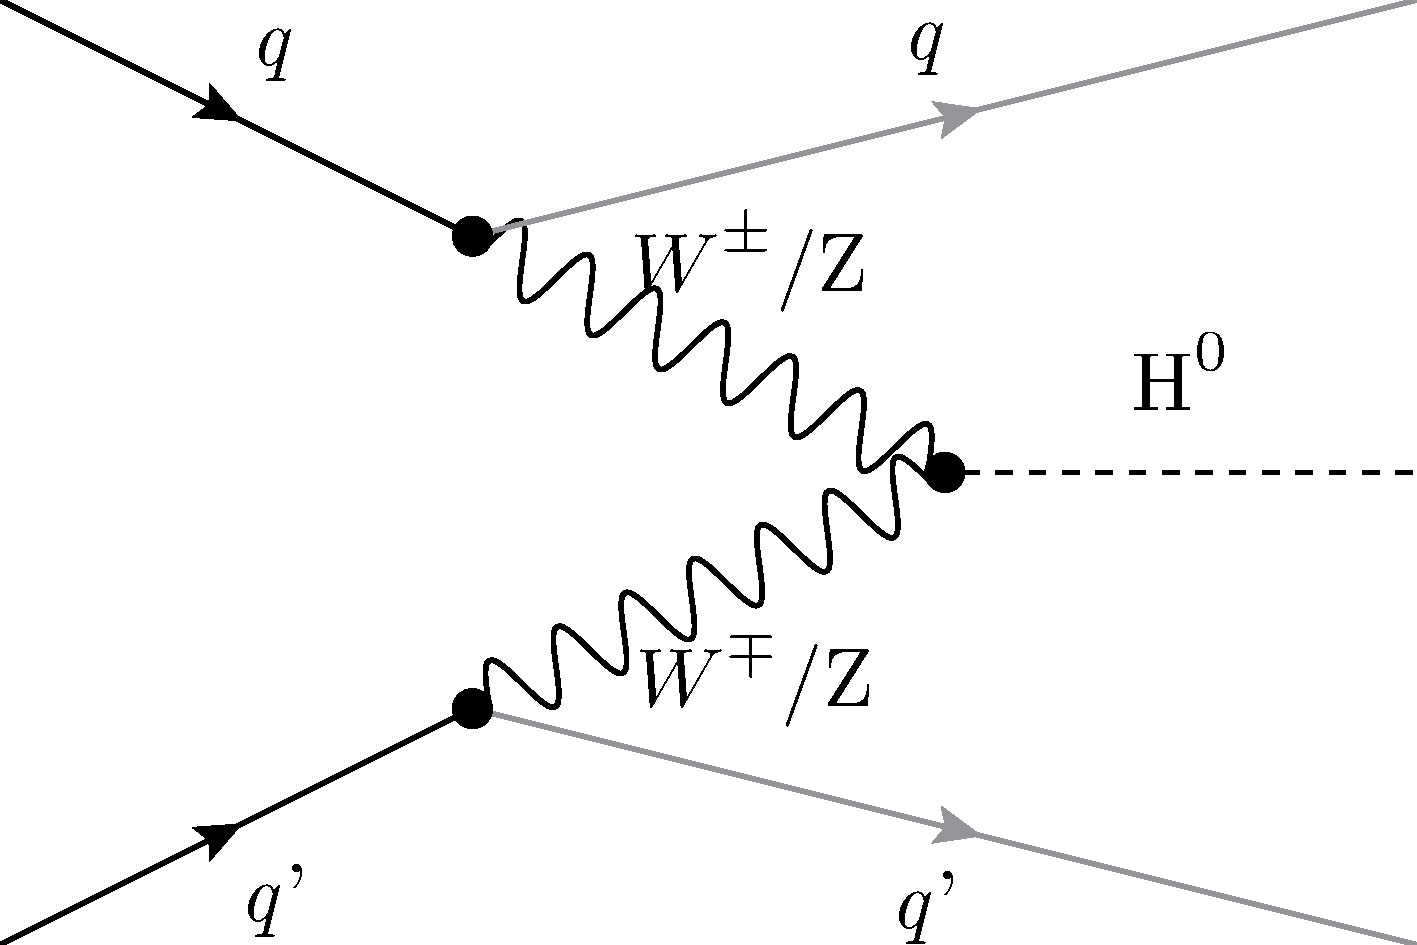
\includegraphics[width=\textwidth]{\figpath/FeynmanDiagrams/qqH.eps}
		\label{fig:qqH}
	\end{subfigure}

	\begin{subfigure}[t]{0.415\textwidth}
		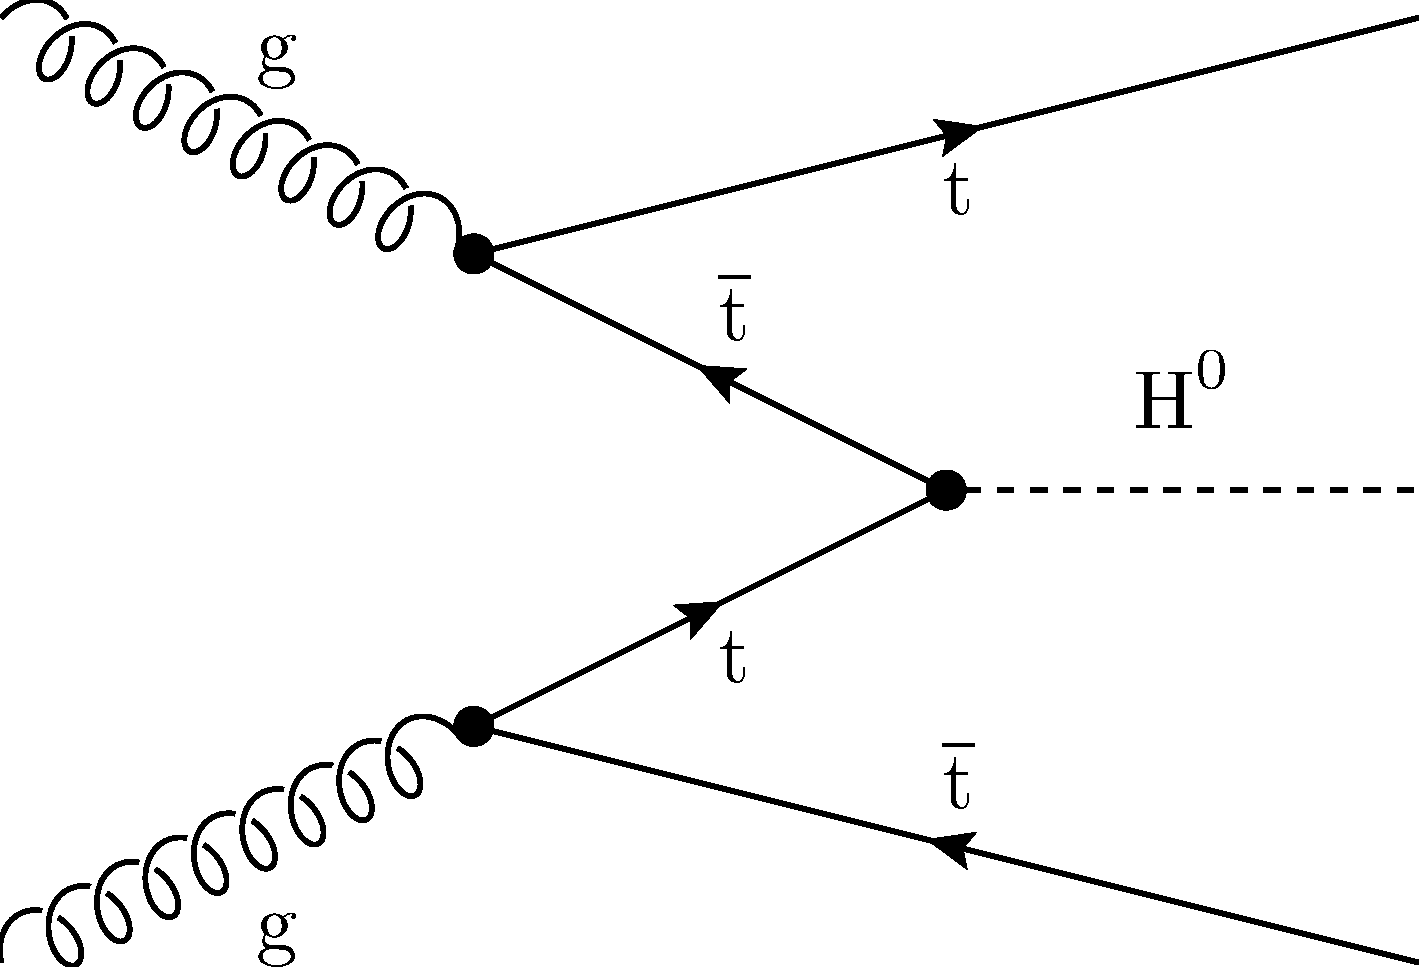
\includegraphics[width=\textwidth]{\figpath/FeynmanDiagrams/ttH.eps}
		\label{fig:ttH}
	\end{subfigure}%
	\begin{subfigure}[t]{0.415\textwidth}
		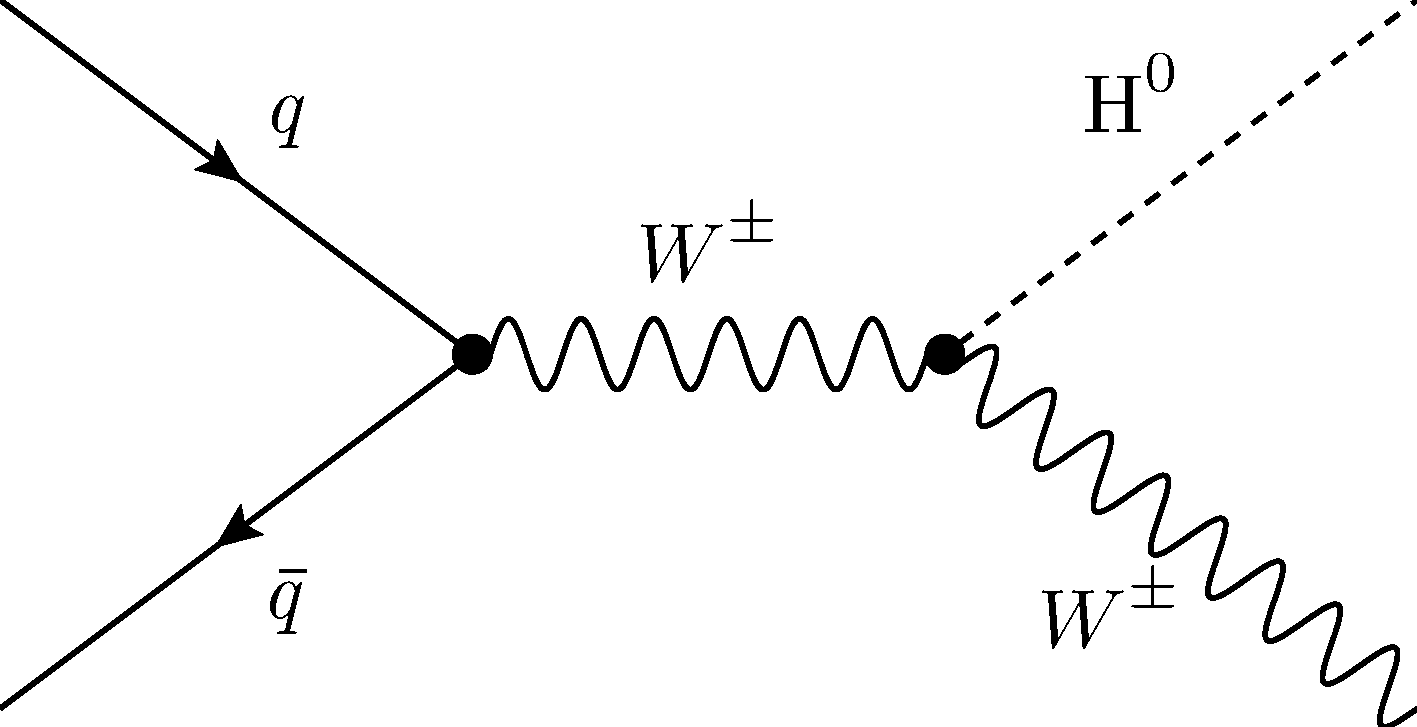
\includegraphics[width=\textwidth]{\figpath/FeynmanDiagrams/WH.eps}
		\label{fig:WH}
	\end{subfigure}
	\caption{Feynman diagrams for the four Higgs production mechanisms with associated $l{\nu}qq$ decays: gluon-gluon fusion (upper left), vector-boson fusion (upper right), \ttbar fusion (lower left), and associated production (lower right).}
	\label{fig:Higgs_WW_lnujj_feynman}
\end{figure}

\begin{figure}[!hbt]
	\centering
	\begin{subfigure}[t]{0.54\textwidth}
		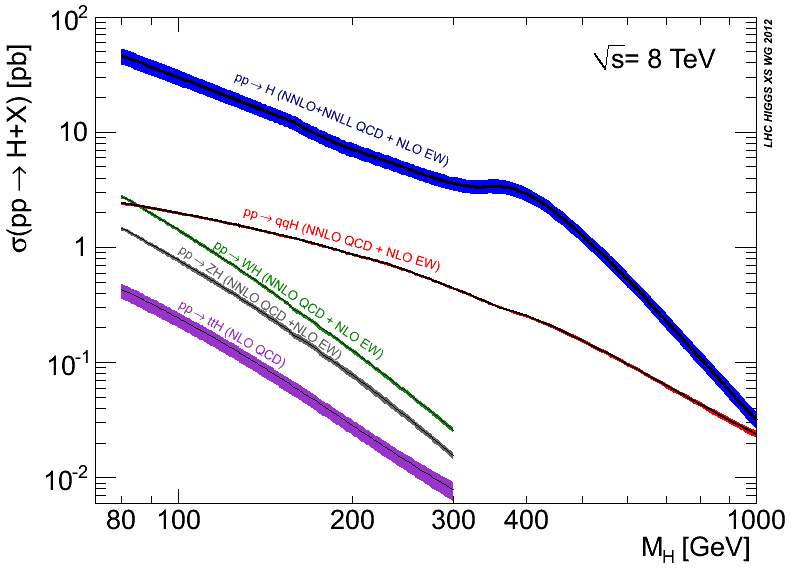
\includegraphics[width=\textwidth]{\figpath/Chapter2/Higgs_XS_8TeV.png}
		\label{fig:Higgs_XS_8TeV}
	\end{subfigure}
	\begin{subfigure}[t]{0.41\textwidth}
		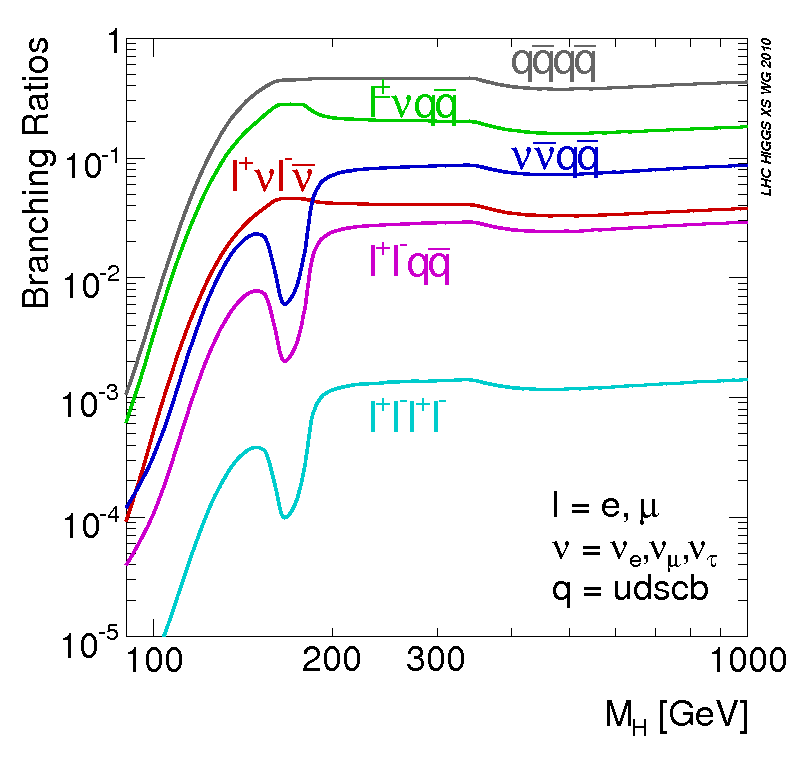
\includegraphics[width=\textwidth]{\figpath/Chapter2/Higgs_BR_4fermion.png}
		\label{fig:Higgs_BR_4fermion}
	\end{subfigure}
	\caption{The Standard Model Higgs production cross sections at 8\tev (left) and WW branching ratios to four fermion final states (right).}
	\label{fig:Higgs_XS_and_BR}
\end{figure}


\section{Beyond the Standard Model}